\documentclass[aspectratio=169,10pt]{beamer}
\usepackage[T1]{fontenc}
\usepackage[utf8]{inputenc}
\usepackage[spanish,es-nodecimaldot]{babel}
\usepackage{lmodern}
\usepackage{amsmath}
\usepackage{booktabs}
\usepackage{graphicx}
\usepackage{tikz}
\usetikzlibrary{arrows.meta,positioning,babel}

% ============================================================
% DATOS DE LA PORTADA (revisar antes de compilar)
% ============================================================
\newcommand{\subtitulo}{Curso opción a tesis}
\newcommand{\fecha}{26 de noviembre de 2026}
\newcommand{\enlace}{https://melanoma.edgar-ontiveros.com}
\newcommand{\enlacecorto}{melanoma.edgar-ontiveros.com}

% ============================================================
% TEMA
% ============================================================
\usetheme{Madrid}
\definecolor{azulfi}{RGB}{11,110,153}
\usecolortheme[named=azulfi]{structure}
\setbeamercolor{block title}{fg=black,bg=azulfi!20}
\setbeamercolor{block body}{bg=azulfi!2}
\setbeamercolor{block title alerted}{fg=white,bg=red!75!black}
\setbeamercolor{block body alerted}{bg=red!75!black!10}
\setbeamercolor{block title example}{fg=white,bg=azulfi!80!black}
\setbeamercolor{block body example}{bg=azulfi!10}
\setbeamerfont{block title}{size=\small}
\setbeamertemplate{navigation symbols}{}
\setbeamertemplate{page number in head/foot}[appendixframenumber]
\setbeamersize{text margin left=3.5mm,text margin right=3.5mm}
\graphicspath{{figuras/}}

% Curvas del sistema final en el conjunto de prueba (datos de reports/f4b_test_results.json)
% Curvas del sistema final (promedio de 3 redes) en el conjunto de prueba.
% Puntos tomados de reports/f4b_test_results.json (curves.roc y curves.pr); no se recalcula nada.
% Ejes: \curvaroc en (1 - especificidad, sensibilidad); \curvapr en (sensibilidad, valor predictivo positivo).
\newcommand{\curvaroc}{(0,0) -- (0.0002,0) -- (0.0004,0) -- (0.0004,0.0116) -- (0.0006,0.0116) -- (0.0006,0.0233) -- (0.0014,0.0233) -- (0.0014,0.0581) -- (0.0025,0.0581) -- (0.0025,0.0698) -- (0.0031,0.0698) -- (0.0031,0.0814) -- (0.0048,0.0814) -- (0.0048,0.093) -- (0.005,0.093) -- (0.005,0.1047) -- (0.0077,0.1047) -- (0.0077,0.1163) -- (0.0081,0.1163) -- (0.0081,0.1279) -- (0.0134,0.1279) -- (0.0134,0.1395) -- (0.0143,0.1395) -- (0.0143,0.1512) -- (0.0153,0.1512) -- (0.0153,0.1628) -- (0.0168,0.1628) -- (0.0168,0.1744) -- (0.018,0.1744) -- (0.018,0.186) -- (0.0201,0.186) -- (0.0201,0.1977) -- (0.0209,0.1977) -- (0.0209,0.2093) -- (0.0213,0.2093) -- (0.0213,0.2209) -- (0.0215,0.2209) -- (0.0215,0.2326) -- (0.0225,0.2326) -- (0.0225,0.2442) -- (0.0275,0.2442) -- (0.0275,0.2558) -- (0.0279,0.2558) -- (0.0279,0.2791) -- (0.0331,0.2791) -- (0.0331,0.2907) -- (0.0346,0.2907) -- (0.0346,0.3023) -- (0.0372,0.3023) -- (0.0372,0.314) -- (0.0389,0.314) -- (0.0389,0.3256) -- (0.0401,0.3256) -- (0.0401,0.3372) -- (0.0405,0.3372) -- (0.0405,0.3488) -- (0.0414,0.3488) -- (0.0414,0.3605) -- (0.0476,0.3605) -- (0.0476,0.3721) -- (0.0494,0.3721) -- (0.0494,0.3953) -- (0.0499,0.3953) -- (0.0499,0.407) -- (0.0538,0.407) -- (0.0538,0.4186) -- (0.0645,0.4186) -- (0.0645,0.4302) -- (0.0674,0.4302) -- (0.0674,0.4419) -- (0.0679,0.4419) -- (0.0679,0.4535) -- (0.0739,0.4535) -- (0.0739,0.4651) -- (0.078,0.4651) -- (0.078,0.4767) -- (0.0813,0.4767) -- (0.0813,0.4884) -- (0.0828,0.4884) -- (0.0828,0.5) -- (0.0875,0.5) -- (0.0875,0.5116) -- (0.0956,0.5116) -- (0.0956,0.5233) -- (0.1014,0.5233) -- (0.1014,0.5349) -- (0.103,0.5349) -- (0.103,0.5465) -- (0.1032,0.5465) -- (0.1032,0.5581) -- (0.1125,0.5581) -- (0.1125,0.5698) -- (0.115,0.5698) -- (0.115,0.5814) -- (0.1152,0.5814) -- (0.1152,0.593) -- (0.1258,0.593) -- (0.1258,0.6047) -- (0.1272,0.6047) -- (0.1272,0.6163) -- (0.1386,0.6163) -- (0.1386,0.6279) -- (0.1465,0.6279) -- (0.1465,0.6395) -- (0.1521,0.6395) -- (0.1521,0.6512) -- (0.1549,0.6512) -- (0.1549,0.6628) -- (0.1597,0.6628) -- (0.1597,0.6744) -- (0.1624,0.6744) -- (0.1624,0.686) -- (0.1731,0.686) -- (0.1731,0.6977) -- (0.1738,0.6977) -- (0.1738,0.7093) -- (0.18,0.7093) -- (0.18,0.7209) -- (0.1829,0.7209) -- (0.1829,0.7326) -- (0.1864,0.7326) -- (0.1864,0.7442) -- (0.1978,0.7442) -- (0.1978,0.7558) -- (0.2017,0.7558) -- (0.2017,0.7674) -- (0.2033,0.7674) -- (0.2033,0.7791) -- (0.2083,0.7791) -- (0.2083,0.7907) -- (0.2096,0.7907) -- (0.2096,0.8023) -- (0.2201,0.8023) -- (0.2201,0.814) -- (0.3128,0.814) -- (0.3132,0.814) -- (0.325,0.814) -- (0.325,0.8256) -- (0.348,0.8256) -- (0.348,0.8372) -- (0.3957,0.8372) -- (0.3957,0.8488) -- (0.4208,0.8488) -- (0.4208,0.8605) -- (0.4487,0.8605) -- (0.4487,0.8721) -- (0.451,0.8721) -- (0.451,0.8837) -- (0.4607,0.8837) -- (0.4607,0.8953) -- (0.4644,0.8953) -- (0.4644,0.907) -- (0.4812,0.907) -- (0.4812,0.9186) -- (0.519,0.9186) -- (0.519,0.9302) -- (0.524,0.9302) -- (0.524,0.9419) -- (0.565,0.9419) -- (0.565,0.9535) -- (0.5687,0.9535) -- (0.5687,0.9651) -- (0.5749,0.9651) -- (0.5749,0.9767) -- (0.6469,0.9767) -- (0.6469,0.9884) -- (0.808,0.9884) -- (0.808,1) -- (0.9766,1) -- (0.977,1) -- (1,1)}
\newcommand{\curvapr}{(0.0116,0.3333) -- (0.0116,0.25) -- (0.0233,0.4) -- (0.0233,0.2222) -- (0.0349,0.3) -- (0.0465,0.3636) -- (0.0581,0.4167) -- (0.0581,0.2778) -- (0.0698,0.3158) -- (0.0698,0.2727) -- (0.0814,0.3043) -- (0.0814,0.2188) -- (0.093,0.2424) -- (0.093,0.2353) -- (0.1047,0.2571) -- (0.1047,0.1837) -- (0.1163,0.2) -- (0.1163,0.1923) -- (0.1279,0.2075) -- (0.1279,0.1375) -- (0.1395,0.1481) -- (0.1395,0.1395) -- (0.1512,0.1494) -- (0.1512,0.1413) -- (0.1628,0.1505) -- (0.1628,0.1386) -- (0.1744,0.1471) -- (0.1744,0.1389) -- (0.186,0.1468) -- (0.186,0.1333) -- (0.1977,0.1405) -- (0.1977,0.136) -- (0.2093,0.1429) -- (0.2093,0.1406) -- (0.2209,0.1473) -- (0.2209,0.1462) -- (0.2326,0.1527) -- (0.2326,0.1471) -- (0.2442,0.1533) -- (0.2442,0.1288) -- (0.2558,0.1341) -- (0.2558,0.1325) -- (0.2674,0.1377) -- (0.2791,0.1429) -- (0.2791,0.1231) -- (0.2907,0.1276) -- (0.2907,0.1225) -- (0.3023,0.1268) -- (0.3023,0.1193) -- (0.314,0.1233) -- (0.314,0.1184) -- (0.3256,0.1223) -- (0.3256,0.1191) -- (0.3372,0.1229) -- (0.3372,0.1218) -- (0.3488,0.1255) -- (0.3488,0.123) -- (0.3605,0.1265) -- (0.3605,0.1119) -- (0.3721,0.1151) -- (0.3721,0.1115) -- (0.3837,0.1146) -- (0.3953,0.1176) -- (0.3953,0.1164) -- (0.407,0.1195) -- (0.407,0.1118) -- (0.4186,0.1146) -- (0.4186,0.0976) -- (0.4302,0.1) -- (0.4302,0.0961) -- (0.4419,0.0984) -- (0.4419,0.0977) -- (0.4535,0.1) -- (0.4535,0.0926) -- (0.4651,0.0948) -- (0.4651,0.0903) -- (0.4767,0.0923) -- (0.4767,0.0889) -- (0.4884,0.0909) -- (0.4884,0.0894) -- (0.5,0.0913) -- (0.5,0.0869) -- (0.5116,0.0887) -- (0.5116,0.0818) -- (0.5233,0.0835) -- (0.5233,0.0791) -- (0.5349,0.0807) -- (0.5349,0.0796) -- (0.5465,0.0812) -- (0.5465,0.081) -- (0.5581,0.0826) -- (0.5581,0.0763) -- (0.5698,0.0778) -- (0.5698,0.0762) -- (0.5814,0.0776) -- (0.5814,0.0775) -- (0.593,0.0789) -- (0.593,0.0728) -- (0.6047,0.0741) -- (0.6047,0.0733) -- (0.6163,0.0746) -- (0.6163,0.0689) -- (0.6279,0.0701) -- (0.6279,0.0666) -- (0.6395,0.0677) -- (0.6395,0.0654) -- (0.6512,0.0665) -- (0.6512,0.0654) -- (0.6628,0.0665) -- (0.6628,0.0646) -- (0.6744,0.0657) -- (0.6744,0.0647) -- (0.686,0.0657) -- (0.686,0.0619) -- (0.6977,0.0629) -- (0.6977,0.0626) -- (0.7093,0.0636) -- (0.7093,0.0616) -- (0.7209,0.0625) -- (0.7209,0.0616) -- (0.7326,0.0625) -- (0.7326,0.0614) -- (0.7442,0.0623) -- (0.7442,0.0589) -- (0.7558,0.0598) -- (0.7558,0.0587) -- (0.7674,0.0596) -- (0.7674,0.0591) -- (0.7791,0.06) -- (0.7791,0.0586) -- (0.7907,0.0594) -- (0.7907,0.0591) -- (0.8023,0.0599) -- (0.8023,0.0572) -- (0.814,0.058) -- (0.814,0.04) -- (0.8256,0.0406) -- (0.8256,0.038) -- (0.8372,0.0385) -- (0.8372,0.034) -- (0.8488,0.0345) -- (0.8488,0.0325) -- (0.8605,0.0329) -- (0.8605,0.0309) -- (0.8721,0.0313) -- (0.8721,0.0312) -- (0.8837,0.0316) -- (0.8837,0.0309) -- (0.8953,0.0313) -- (0.8953,0.0311) -- (0.907,0.0315) -- (0.907,0.0304) -- (0.9186,0.0308) -- (0.9186,0.0286) -- (0.9302,0.029) -- (0.9302,0.0287) -- (0.9419,0.0291) -- (0.9419,0.027) -- (0.9535,0.0273) -- (0.9535,0.0272) -- (0.9651,0.0275) -- (0.9651,0.0272) -- (0.9767,0.0275) -- (0.9767,0.0245) -- (0.9884,0.0248) -- (0.9884,0.02) -- (1,0.0202) -- (1,0.0164)}


% Cifras clave en grande y notas al pie de lámina
\newcommand{\cifra}[1]{{\fontsize{24}{26}\selectfont\bfseries\color{azulfi}#1}}
\newcommand{\cifram}[1]{{\fontsize{16}{18}\selectfont\bfseries\color{azulfi}#1}}
\newcommand{\nota}[1]{{\footnotesize\color{black!65}#1}}

\tikzset{
  caja/.style={draw=azulfi,rounded corners=1pt,font=\footnotesize,align=center,inner sep=3.5pt,minimum height=9mm,minimum width=2.1cm},
  cajallena/.style={caja,fill=azulfi,text=white},
  cajasuave/.style={caja,fill=azulfi!10},
  flecha/.style={-{Stealth[length=1.8mm]},azulfi,thick},
  celda/.style={minimum width=2.9cm,minimum height=1.45cm,align=center,font=\footnotesize,inner sep=2pt},
  acierto/.style={celda,fill=azulfi!18},
  error/.style={celda,fill=red!75!black!14}
}

\title[Detección asistida de melanoma]{Detección asistida de melanoma en imágenes dermatoscópicas con redes neuronales convolucionales}
\subtitle{\subtitulo}
\author[E. E. Ontiveros Lara]{Edgar Eduardo Ontiveros Lara}
\institute[UACH]{Ingeniería Física\\Facultad de Ingeniería\\Universidad Autónoma de Chihuahua}
\date[\fecha]{\fecha}
\titlegraphic{%
  \href{\enlace}{\texttt{\enlace}}\\[0.9em]
  
\includegraphics[height=13mm]{logo_uach}\hspace{6.8cm}
\includegraphics[height=13mm]{logo_fi}%
}

\begin{document}

% ============================================================
% 1. PORTADA
% ============================================================
\begin{frame}[plain]
  \titlepage
\end{frame}

% ============================================================
% 2. EL PROBLEMA Y EL OBJETIVO
% ============================================================
\begin{frame}{El problema y el objetivo}
  \begin{columns}[T]
    \begin{column}{0.48\textwidth}
      \begin{block}{El problema}
        En el conjunto ISIC 2020, solo \textbf{1 de cada 57} dermatoscopías es un melanoma.\\[0.3em]
        Hay que encontrar pocos casos entre muchos, sin dejarlos pasar.
      \end{block}
    \end{column}
    \begin{column}{0.48\textwidth}
      \begin{block}{El objetivo}
        Construir y medir un sistema que \textbf{detecte} las dermatoscopías con sospecha de melanoma y recomiende \textbf{referirlas} a dermatología.
      \end{block}
    \end{column}
  \end{columns}
  \vspace{0.1em}
  \begin{center}
    \begin{tikzpicture}[node distance=7mm]
      \node[caja] (img) {Dermatoscopía};
      \node[cajallena,right=of img] (sis) {Sistema};
      \node[cajasuave,right=11mm of sis,minimum width=4.8cm,minimum height=6.5mm] (rec) {Recomendación: \textbf{referir} o \textbf{no referir}};
      \node[cajasuave,above=1.2mm of rec,minimum width=4.8cm,minimum height=6.5mm] (pro) {Probabilidad de melanoma};
      \node[cajasuave,below=1.2mm of rec,minimum width=4.8cm,minimum height=6.5mm] (map) {Mapa de activación};
      \draw[flecha] (img) -- (sis);
      \draw[flecha] (sis.east) -- (rec.west);
      \draw[flecha] (sis.east) -- ++(4mm,0) |- (pro.west);
      \draw[flecha] (sis.east) -- ++(4mm,0) |- (map.west);
    \end{tikzpicture}
  \end{center}
  \vspace{-0.3em}
  \begin{alertblock}{El sistema detecta, no diagnostica}
    Entrega una probabilidad y una recomendación. \textbf{La decisión es del médico.}
  \end{alertblock}
\end{frame}

% ============================================================
% 3. LOS DATOS
% ============================================================
\begin{frame}{Los datos: ISIC 2020 y el reparto por paciente}
  \begin{columns}[c]
    \begin{column}{0.31\textwidth}\centering
      \cifra{33,126}\\ dermatoscopías
    \end{column}
    \begin{column}{0.31\textwidth}\centering
      \cifra{2,056}\\ pacientes
    \end{column}
    \begin{column}{0.31\textwidth}\centering
      \cifra{584}\\ melanomas (\textbf{1.76\,\%})
    \end{column}
  \end{columns}
  \vspace{1.1em}
  \begin{center}
    \begin{tikzpicture}[node distance=7mm and 6mm]
      \node[caja,minimum width=4.4cm] (val) {\textbf{Validación}\\4,963 imágenes · 88 melanomas\\\emph{tomar decisiones}};
      \node[caja,left=of val,minimum width=4.4cm] (ent) {\textbf{Entrenamiento}\\22,911 imágenes · 410 melanomas\\\emph{ajustar los pesos}};
      \node[cajallena,right=of val,minimum width=4.4cm] (pru) {\textbf{Prueba}\\5,252 imágenes · 86 melanomas\\\emph{medición final}};
      \node[cajasuave,above=8mm of val,minimum width=6.2cm] (todo) {Reparto \textbf{por paciente}};
      \draw[flecha] (todo.south) -- (val.north);
      \draw[flecha] (todo.south) -- ++(0,-4mm) -| (ent.north);
      \draw[flecha] (todo.south) -- ++(0,-4mm) -| (pru.north);
    \end{tikzpicture}
  \end{center}
  \vspace{0.6em}
  \begin{itemize}
    \item Ningún paciente aparece en dos conjuntos: el sistema no puede reconocer al paciente en lugar de la lesión.
    \item El conjunto de prueba se abrió \textbf{solo dos veces} en todo el proyecto.
  \end{itemize}
\end{frame}

% ============================================================
% 4. EL MODELO
% ============================================================
\begin{frame}{El modelo: EfficientNetV2-S y transfer learning}
  \begin{center}
    \begin{tikzpicture}[node distance=6mm]
      \node[caja,minimum width=2.8cm] (inet) {\textbf{ImageNet}\\pesos iniciales};
      \node[cajallena,right=of inet,minimum width=3.2cm] (red) {\textbf{EfficientNetV2-S}\\red convolucional};
      \node[caja,right=of red,minimum width=3.0cm] (fino) {\textbf{Ajuste fino}\\de toda la red};
      \node[cajasuave,right=of fino,minimum width=3.4cm] (sal) {\textbf{Salida}\\probabilidad de melanoma};
      \foreach \a/\b in {inet/red,red/fino,fino/sal} \draw[flecha] (\a) -- (\b);
    \end{tikzpicture}
  \end{center}
  \vspace{0.8em}
  \begin{columns}[c]
    \begin{column}{0.30\textwidth}\centering
      \cifra{20.2}\\ millones de parámetros
    \end{column}
    \begin{column}{0.30\textwidth}\centering
      \cifra{224}\\ píxeles por lado
    \end{column}
    \begin{column}{0.30\textwidth}\centering
      \cifra{22,911}\\ dermatoscopías de ajuste
    \end{column}
  \end{columns}
  \vspace{1.0em}
  \begin{itemize}
    \item \textbf{Transfer learning}: la red ya sabe reconocer formas y texturas; se ajusta a la dermatoscopía.
    \item Solo hay \textbf{410 melanomas} para entrenar; por eso se parte de una red ya entrenada.
    \item Red de Tan y Le (2021). Se ajustan todos sus pesos, no solo la última capa.
  \end{itemize}
\end{frame}

% ============================================================
% 5. EL ENTRENAMIENTO
% ============================================================
\begin{frame}{El entrenamiento}
  \begin{columns}[T]
    \begin{column}{0.31\textwidth}
      \begin{block}{La receta}
        \begin{itemize}
          \item Optimizador AdamW
          \item Tasa de aprendizaje 0.0001, con calentamiento de 1 época y coseno
          \item Lotes de 128 imágenes
          \item Máximo 15 épocas
          \item 3 semillas
          \item Tesla T4 de Kaggle
        \end{itemize}
      \end{block}
    \end{column}
    \begin{column}{0.31\textwidth}
      \begin{exampleblock}{El peso de los melanomas}
        \centering
        \cifra{54.88}\\[0.3em]
        \raggedright
        En entrenamiento hay 54.88 lesiones benignas por cada melanoma.\\[0.3em]
        En la pérdida (entropía cruzada binaria), fallar en un melanoma cuesta \textbf{54.88 veces más}.
      \end{exampleblock}
    \end{column}
    \begin{column}{0.31\textwidth}
      \begin{block}{Frenos contra la memorización}
        \begin{itemize}
          \item Parada temprana: paciencia de 5 épocas sobre el AUPRC de validación
          \item Decaimiento de pesos 0.01
          \item Dropout 0.2
          \item Aumentos de datos: recorte, volteos, rotación de $\pm 20^{\circ}$, brillo y contraste
        \end{itemize}
      \end{block}
    \end{column}
  \end{columns}
\end{frame}

% ============================================================
% 6. LA ELECCION DEL MODELO
% ============================================================
\begin{frame}{La elección del modelo}
  \begin{columns}[c]
    \begin{column}{0.57\textwidth}
      \centering
      \begin{tikzpicture}[x=11.5cm,y=0.92cm]
        \foreach \nombre/\detalle/\valor/\fila/\tono in {
          Sin imagen/solo datos del paciente/0.620/4/azulfi!30,
          ResNet50/224 píxeles/0.778/3/azulfi!30,
          EfficientNetV2-S/224 píxeles/0.825/2/azulfi,
          EfficientNetV2-S/384 píxeles/0.829/1/azulfi!30,
          ConvNeXt-Tiny/384 píxeles/0.833/0/azulfi!30}{
          \fill[fill=\tono] (0.5,\fila-0.3) rectangle (\valor,\fila+0.3);
          \node[anchor=east,font=\footnotesize,align=right,inner sep=2pt] at (0.495,\fila) {\textbf{\nombre}\\[-0.2em]{\scriptsize \detalle}};
          \node[anchor=west,font=\footnotesize\bfseries] at (\valor,\fila) {\valor};
        }
        \draw[black!55] (0.5,-0.55) -- (0.5,4.55);
        \node[anchor=north,font=\scriptsize,black!65] at (0.5,-0.55) {0.5 = azar};
        \draw[black!60,thick] (0.905,-0.3) -- (0.912,-0.3) -- (0.912,2.3) -- (0.905,2.3);
        \node[anchor=west,font=\scriptsize] at (0.914,1) {empate};
      \end{tikzpicture}\\[0.2em]
      \nota{AUC-ROC en validación. Redes: media de 3 semillas.}
    \end{column}
    \begin{column}{0.40\textwidth}
      \begin{block}{Primero se midió el ruido}
        El mismo entrenamiento, repetido, dio \textbf{0.794} y \textbf{0.778}.
      \end{block}
      \begin{block}{La regla, fijada de antemano}
        Diferencias menores a \textbf{0.02} son empate.\\
        En un empate gana el modelo más barato.
      \end{block}
      \begin{exampleblock}{Elegido}
        \textbf{EfficientNetV2-S a 224 píxeles}: empata con los dos mayores y cuesta 4.5 veces menos cómputo que ConvNeXt-Tiny.
      \end{exampleblock}
    \end{column}
  \end{columns}
\end{frame}

% ============================================================
% 7. EL SISTEMA FINAL
% ============================================================
\begin{frame}{El sistema final}
  \begin{center}
    \begin{tikzpicture}[node distance=4mm]
      \node[caja,minimum width=2.2cm] (img) {Dermatoscopía};
      \node[caja,right=of img,minimum width=2.7cm] (ens) {3 redes\\EfficientNetV2-S};
      \node[caja,right=of ens,minimum width=1.7cm] (avg) {Promedio};
      \node[caja,right=of avg,minimum width=2.0cm] (cal) {Calibración\\de Platt};
      \node[caja,right=of cal,minimum width=1.6cm] (thr) {Umbral\\0.39\,\%};
      \node[cajallena,right=of thr,minimum width=2.1cm] (out) {Referir o\\no referir};
      \foreach \a/\b in {img/ens,ens/avg,avg/cal,cal/thr,thr/out} \draw[flecha] (\a) -- (\b);
    \end{tikzpicture}
  \end{center}
  \vspace{0.6em}
  \begin{columns}[T]
    \begin{column}{0.31\textwidth}
      \begin{block}{Ensamble}
        \centering\cifram{3 redes}\\[0.2em]
        \raggedright
        La misma red, entrenada con 3 semillas.\\[0.2em]
        En validación, el AUC-ROC sube de \textbf{0.834} a \textbf{0.847}.
      \end{block}
    \end{column}
    \begin{column}{0.31\textwidth}
      \begin{block}{Calibración de Platt}
        \centering\cifram{2 parámetros}\\[0.2em]
        \raggedright
        $a = 0.4473$ y $b = -3.3553$, ajustados en validación.\\[0.2em]
        La probabilidad se lee tal cual: 8\,\% quiere decir 8 de cada 100.
      \end{block}
    \end{column}
    \begin{column}{0.31\textwidth}
      \begin{exampleblock}{Umbral}
        \centering\cifram{0.39\,\%}\\[0.2em]
        \raggedright
        Fijado en validación para detectar \textbf{al menos 95\,\%} de los melanomas.\\[0.2em]
        Probabilidad mayor: referir.
      \end{exampleblock}
    \end{column}
  \end{columns}
\end{frame}

% ============================================================
% 8. RESULTADOS: MATRIZ DE CONFUSION
% ============================================================
\begin{frame}{Resultados en prueba: matriz de confusión}
  \begin{columns}[c]
    \begin{column}{0.56\textwidth}
      \centering
      \begin{tikzpicture}
        \node[acierto] (tp) at (0,0) {{\LARGE\bfseries 84}\\detectados};
        \node[error]   (fn) at (3.0,0) {{\LARGE\bfseries 2}\\no detectados};
        \node[error]   (fp) at (0,-1.55) {{\LARGE\bfseries 3,138}\\falsas alarmas};
        \node[acierto] (tn) at (3.0,-1.55) {{\LARGE\bfseries 2,028}\\bien descartadas};
        \node[font=\footnotesize\bfseries,above=1mm of tp] {El sistema refirió};
        \node[font=\footnotesize\bfseries,above=1mm of fn] {No refirió};
        \node[font=\footnotesize,anchor=east,align=right] at (-1.6,0) {\textbf{Melanoma}\\86 lesiones};
        \node[font=\footnotesize,anchor=east,align=right] at (-1.6,-1.55) {\textbf{Lesión benigna}\\5,166 lesiones};
      \end{tikzpicture}\\[0.6em]
      \nota{5,252 dermatoscopías de 540 pacientes. Umbral de 0.39\,\%.}
    \end{column}
    \begin{column}{0.41\textwidth}
      \begin{columns}[c]
        \begin{column}{0.48\textwidth}\centering
          \cifra{97.7\,\%}\\ sensibilidad\\ \nota{84 de 86}
        \end{column}
        \begin{column}{0.48\textwidth}\centering
          \cifra{39.3\,\%}\\ especificidad\\ \nota{2,028 de 5,166}
        \end{column}
      \end{columns}
      \vspace{1.2em}
      \begin{columns}[c]
        \begin{column}{0.48\textwidth}\centering
          \cifra{2.6\,\%}\\ valor predictivo positivo\\ \nota{84 de 3,222}
        \end{column}
        \begin{column}{0.48\textwidth}\centering
          \cifra{99.9\,\%}\\ valor predictivo negativo\\ \nota{2,028 de 2,030}
        \end{column}
      \end{columns}
    \end{column}
  \end{columns}
\end{frame}

% ============================================================
% 9. RESULTADOS: AUC-ROC Y AUPRC
% ============================================================
\begin{frame}{Resultados en prueba: AUC-ROC y AUPRC}
  \begin{columns}[c]
    \begin{column}{0.34\textwidth}
      \centering
      \begin{tikzpicture}[x=3.85cm,y=3.85cm]
        \fill[azulfi!12] \curvaroc -- (1,0) -- cycle;
        \draw[black!45,dashed] (0,0) -- (1,1);
        \draw[azulfi,very thick,line join=round] \curvaroc;
        \draw[black!70] (0,0) rectangle (1,1);
        \foreach \t in {0,0.5,1} {
          \node[below,font=\scriptsize] at (\t,0) {\t};
          \node[left,font=\scriptsize] at (0,\t) {\t};
        }
        \node[font=\scriptsize] at (0.5,-0.2) {1 $-$ especificidad};
        \node[font=\scriptsize,rotate=90] at (-0.23,0.5) {Sensibilidad};
        \node[font=\scriptsize,black!60,rotate=45] at (0.66,0.58) {azar};
      \end{tikzpicture}\\[0.1em]
      {\footnotesize\textbf{Curva ROC}}
    \end{column}
    \begin{column}{0.34\textwidth}
      \centering
      \begin{tikzpicture}[x=3.85cm,y=7.7cm]
        \begin{scope}
          \clip (0,0) rectangle (1,0.5);
          \draw[azulfi,very thick,line join=round] \curvapr;
          \draw[black!45,dashed] (0,0.0164) -- (1,0.0164);
        \end{scope}
        \draw[black!70] (0,0) rectangle (1,0.5);
        \foreach \t in {0,0.5,1} \node[below,font=\scriptsize] at (\t,0) {\t};
        \foreach \t in {0,0.25,0.5} \node[left,font=\scriptsize] at (0,\t) {\t};
        \node[font=\scriptsize] at (0.5,-0.1) {Sensibilidad};
        \node[font=\scriptsize,rotate=90] at (-0.27,0.25) {Valor predictivo positivo};
        \node[font=\scriptsize,black!60,anchor=south west] at (0.03,0.02) {azar: 0.016};
      \end{tikzpicture}\\[0.1em]
      {\footnotesize\textbf{Curva de precisión y sensibilidad}}
    \end{column}
    \begin{column}{0.27\textwidth}
      {\small\textbf{AUC-ROC}}\\[0.2em]
      \cifra{0.843}\\[0.1em]
      \nota{intervalo del 95\,\%:\\0.804 a 0.881}\\[1.1em]
      {\small\textbf{AUPRC}}\\[0.2em]
      \cifra{0.113}\\[0.1em]
      \nota{intervalo del 95\,\%:\\0.076 a 0.179}\\[0.9em]
      {\small \textbf{7 veces} el azar}
    \end{column}
  \end{columns}
  \vspace{0.2em}
  \begin{center}
    \nota{AUC-ROC y AUPRC son las áreas bajo cada curva. Intervalos del 95\,\% por remuestreo de pacientes.}
  \end{center}
\end{frame}

% ============================================================
% 10. POR QUE LA ESPECIFICIDAD ES BAJA
% ============================================================
\begin{frame}{Por qué la especificidad es baja}
  \begin{block}{El umbral se fijó para no dejar ir melanomas}
    Se fijó en validación, antes de medir el sistema en la prueba, con una sola condición: detectar \textbf{al menos 95\,\%} de los melanomas.
  \end{block}
  \vspace{0.4em}
  \begin{columns}[T]
    \begin{column}{0.36\textwidth}
      \begin{exampleblock}{Umbral elegido: 0.39\,\%}
        \centering
        \cifram{84 de 86}\\ melanomas detectados\\[0.4em]
        \cifram{39.3\,\%}\\ de especificidad
      \end{exampleblock}
    \end{column}
    \begin{column}{0.36\textwidth}
      \begin{block}{Umbral más alto: 0.56\,\%}
        \centering
        \cifram{74 de 86}\\ melanomas detectados\\[0.4em]
        \cifram{55.7\,\%}\\ de especificidad
      \end{block}
    \end{column}
    \begin{column}{0.22\textwidth}
      \centering
      \begin{tikzpicture}[x=2.65cm,y=2.65cm]
        \draw[black!45,dashed] (0,0) -- (1,1);
        \draw[azulfi,thick,line join=round] \curvaroc;
        \draw[black!70] (0,0) rectangle (1,1);
        \fill[white,draw=azulfi!70!black,thick] (0.4429,0.8605) circle (1.6pt);
        \fill[red!75!black] (0.6074,0.9767) circle (2pt);
        \fill[red!75!black] (0.56,0.30) circle (2pt);
        \node[font=\scriptsize,anchor=west,inner sep=1pt] at (0.61,0.30) {0.39\,\%};
        \fill[white,draw=azulfi!70!black,thick] (0.56,0.15) circle (1.6pt);
        \node[font=\scriptsize,anchor=west,inner sep=1pt] at (0.61,0.15) {0.56\,\%};
        \node[font=\scriptsize] at (0.5,-0.12) {1 $-$ especificidad};
        \node[font=\scriptsize,rotate=90] at (-0.12,0.5) {Sensibilidad};
      \end{tikzpicture}
    \end{column}
  \end{columns}
  \vspace{0.3em}
  \begin{itemize}
    \item Subir el umbral mejora la especificidad, pero deja ir \textbf{12 melanomas en lugar de 2}.
    \item Con el umbral elegido se refiere el \textbf{61\,\%} de las lesiones: el sistema sirve para \textbf{priorizar}, no para descartar.
  \end{itemize}
\end{frame}

% ============================================================
% 11. LIMITES
% ============================================================
\begin{frame}{Límites}
  \begin{columns}[c]
    \begin{column}{0.62\textwidth}
      \begin{enumerate}
        \item \textbf{Solo dermatoscopías.} Con 656 fotografías clínicas, el AUC-ROC cayó a 0.596.
        \item \textbf{Pocos melanomas en la prueba.} Son 86: el intervalo del AUC-ROC mide $\pm 0.04$.
        \item \textbf{No verifica el tipo de imagen.} Cualquier imagen recibe una probabilidad.
        \item \textbf{El mapa de activación no explica la decisión.} Muestra dónde se apoyó la red, no por qué.
        \item \textbf{Prototipo de investigación.} Sin validación clínica ni aprobación regulatoria.
      \end{enumerate}
    \end{column}
    \begin{column}{0.34\textwidth}
      \centering
      \begin{tikzpicture}[x=1.7cm,y=6.2cm]
        \draw[black!55] (-0.6,0.5) -- (1.6,0.5);
        \fill[azulfi] (-0.35,0.5) rectangle (0.35,0.834);
        \fill[red!75!black!70] (0.65,0.5) rectangle (1.35,0.596);
        \node[above,font=\small\bfseries] at (0,0.834) {0.834};
        \node[above,font=\small\bfseries] at (1,0.596) {0.596};
        \node[below,font=\scriptsize,align=center] at (0,0.5) {Dermatoscopías\\de prueba};
        \node[below,font=\scriptsize,align=center] at (1,0.5) {Fotografías\\clínicas};
        \node[left,font=\scriptsize,black!65] at (-0.6,0.5) {azar};
      \end{tikzpicture}\\[0.3em]
      \nota{AUC-ROC de una sola red}
    \end{column}
  \end{columns}
\end{frame}

% ============================================================
% 12. EL PRODUCTO Y LA DEMOSTRACION
% ============================================================
\begin{frame}{El producto y la demostración}
  \begin{columns}[c]
    \begin{column}{0.47\textwidth}
      \centering
      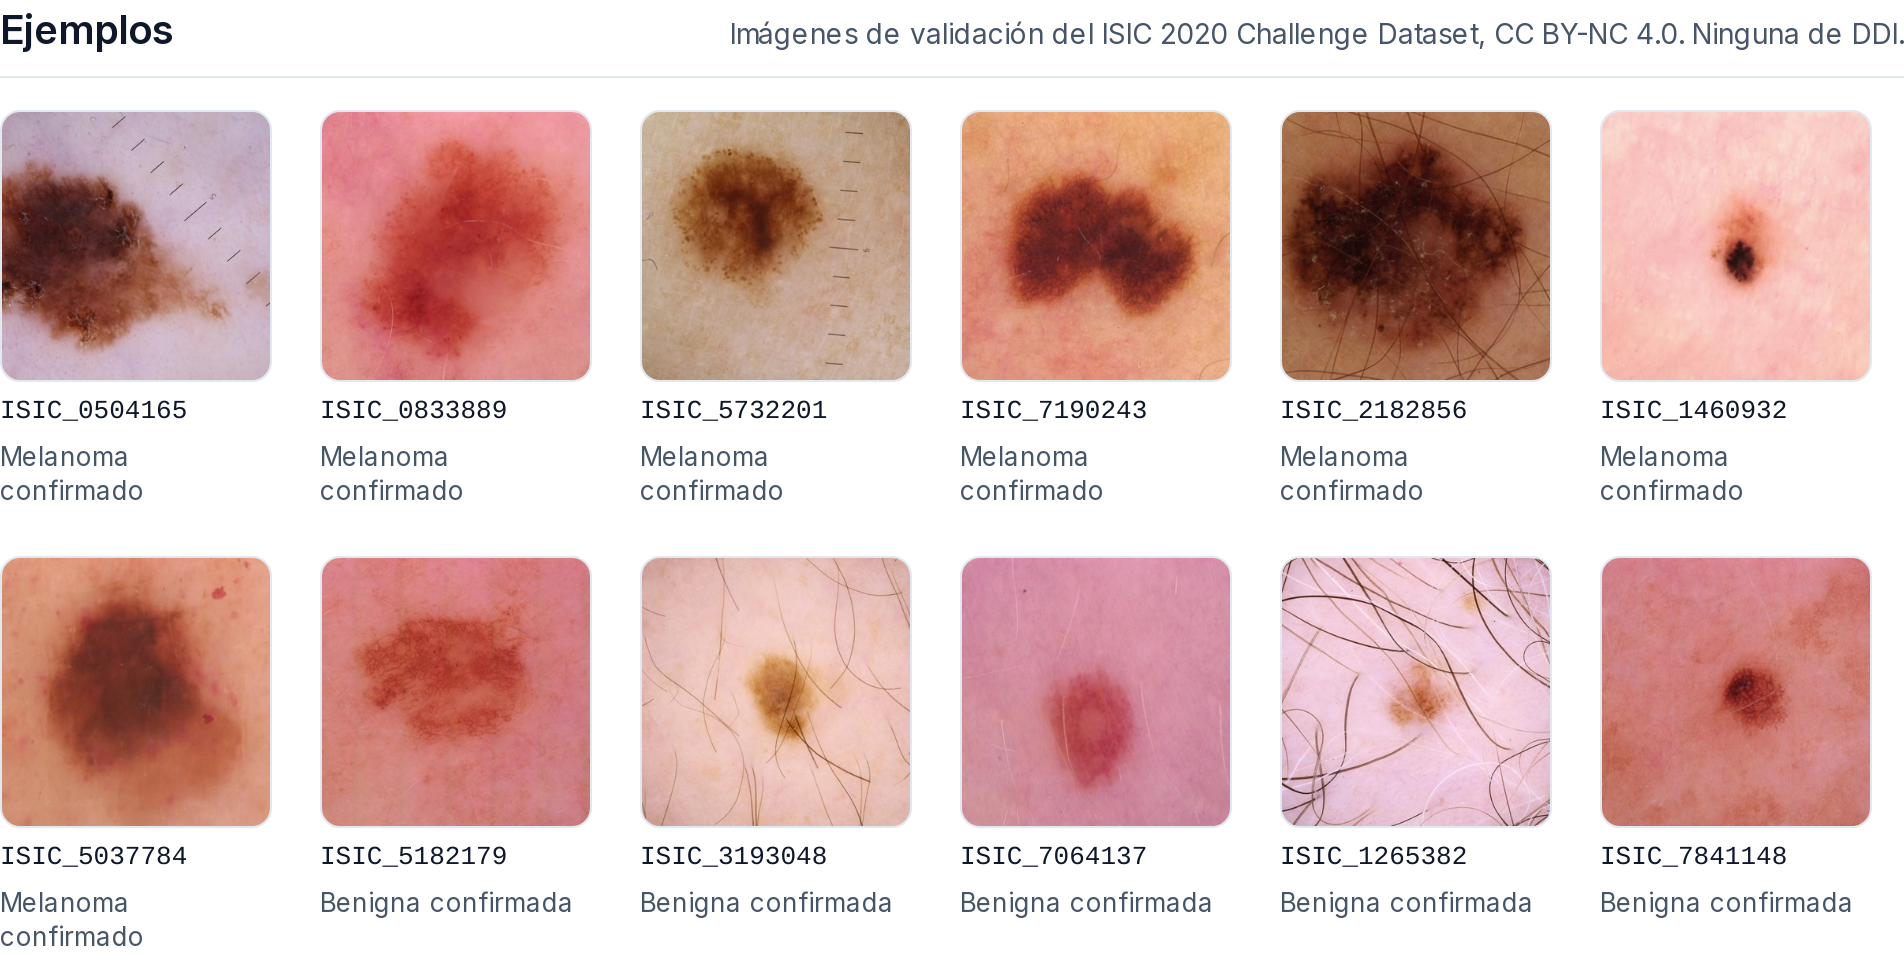
\includegraphics[width=\linewidth]{ui_galeria}\\[0.2em]
      \nota{12 ejemplos de validación}
    \end{column}
    \begin{column}{0.29\textwidth}
      \centering
      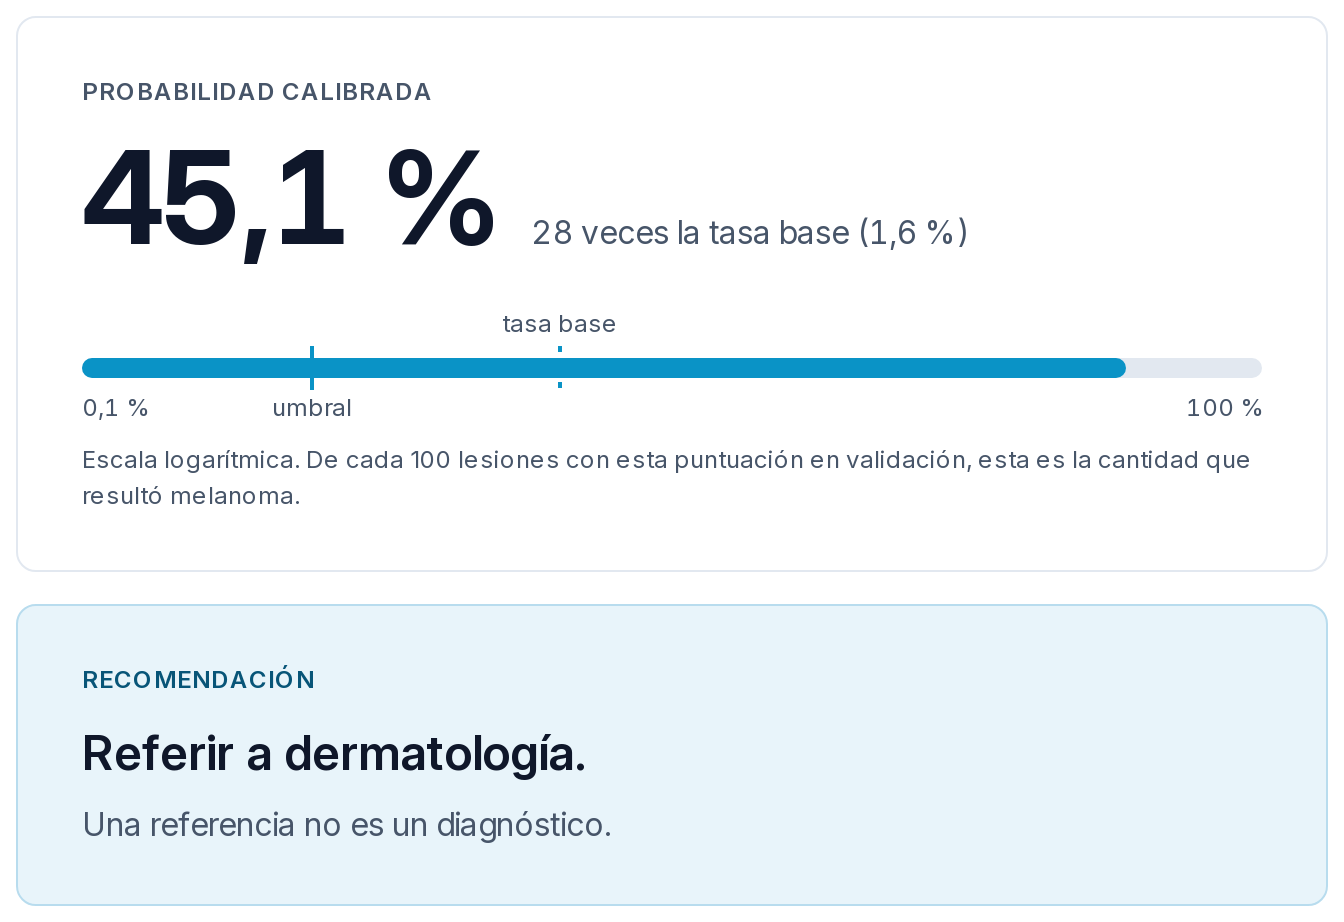
\includegraphics[width=\linewidth]{ui_resultado}\\[0.2em]
      \nota{Probabilidad y recomendación}
    \end{column}
    \begin{column}{0.19\textwidth}
      \centering
      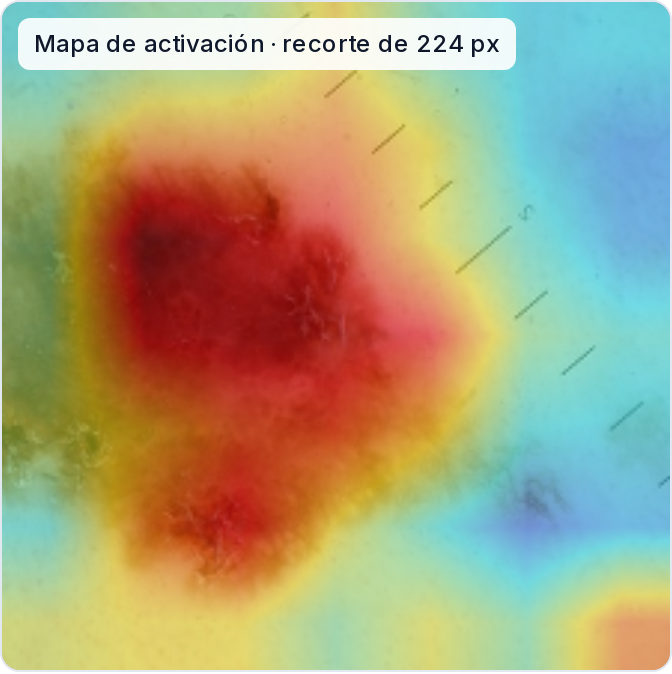
\includegraphics[width=\linewidth]{ui_mapa}\\[0.2em]
      \nota{Mapa de activación}
    \end{column}
  \end{columns}
  \vspace{0.9em}
  \begin{center}
    {\Large\bfseries\href{\enlace}{\texttt{\enlace}}}\\[0.5em]
    Página pública. Responde en \textbf{99 milisegundos} por imagen, sin tarjeta gráfica.
  \end{center}
\end{frame}

% ============================================================
% 13. APORTACION Y CONCLUSIONES
% ============================================================
\begin{frame}{Aportación y conclusiones}
  \begin{block}{Aportación}
    Un sistema completo y \textbf{medido de principio a fin}: reparto por paciente, conjunto de prueba abierto solo dos veces, probabilidades calibradas y una página pública para probarlo.
  \end{block}
  \vspace{0.5em}
  \begin{columns}[c]
    \begin{column}{0.30\textwidth}\centering
      \cifra{84 de 86}\\ melanomas detectados
    \end{column}
    \begin{column}{0.30\textwidth}\centering
      \cifra{0.843}\\ AUC-ROC en prueba
    \end{column}
    \begin{column}{0.30\textwidth}\centering
      \cifra{39.3\,\%}\\ de especificidad
    \end{column}
  \end{columns}
  \vspace{0.8em}
  \begin{itemize}
    \item Detecta casi todos los melanomas; el costo son muchas falsas alarmas.
    \item Sirve para \textbf{priorizar} a quién referir, no para descartar.
    \item Fuera de la dermatoscopía no funciona.
  \end{itemize}
  \begin{exampleblock}{En una frase}
    El sistema \textbf{detecta, no diagnostica}.
  \end{exampleblock}
\end{frame}

% ============================================================
% 14. TRABAJO FUTURO
% ============================================================
\begin{frame}{Trabajo futuro}
  \begin{itemize}
    \setlength{\itemsep}{0.9em}
    \item \textbf{Más melanomas.} Sumar otros años de ISIC, cuidando el reparto por paciente.
    \item \textbf{Verificar el tipo de imagen.} Rechazar lo que no sea una dermatoscopía antes de responder.
    \item \textbf{Resistir artefactos.} Recortar o segmentar la lesión antes de clasificar.
    \item \textbf{Validación local.} Medirlo con pacientes mexicanos y con el equipo de una clínica.
    \item \textbf{Un conjunto de prueba nuevo.} El actual ya se abrió dos veces: cualquier mejora necesita datos nuevos para medirse.
  \end{itemize}
\end{frame}

% ============================================================
% 15. CIERRE
% ============================================================
\begin{frame}[plain]
  \begin{center}
    {\huge\bfseries\color{azulfi} Gracias}\\[1.0em]
    {\Large ¿Preguntas?}\\[1.8em]
    {\Large\bfseries\href{\enlace}{\texttt{\enlace}}}\\[1.8em]
    \textbf{Edgar Eduardo Ontiveros Lara}\\[0.3em]
    \small Ingeniería Física --- Facultad de Ingeniería --- Universidad Autónoma de Chihuahua\\[2.0em]
    
\includegraphics[height=12mm]{logo_uach}\hspace{6.8cm}
\includegraphics[height=12mm]{logo_fi}
  \end{center}
\end{frame}

% ============================================================
% LAMINAS DE RESPALDO (no cuentan en las 15)
% ============================================================
\appendix

\begin{frame}{Respaldo: la receta completa de entrenamiento}
  \begin{center}
    \small
    \begin{tabular}{ll}
      \toprule
      \textbf{Elemento} & \textbf{Valor} \\
      \midrule
      Red & EfficientNetV2-S, 20.2 millones de parámetros, pesos iniciales de ImageNet \\
      Entrada & Imágenes de 224 píxeles \\
      Ajuste & Fino, de toda la red \\
      Pérdida & Entropía cruzada binaria, peso de 54.88 para los melanomas \\
      Optimizador & AdamW, decaimiento de pesos 0.01 \\
      Tasa de aprendizaje & 0.0001, calentamiento de 1 época y coseno \\
      Lotes & 128 imágenes \\
      Duración & Máximo 15 épocas; parada temprana con paciencia 5 sobre el AUPRC de validación \\
      Regularización & Dropout 0.2 \\
      Aumentos de datos & Recorte, volteos, rotación de $\pm 20^{\circ}$, brillo y contraste \\
      Repeticiones & 3 semillas \\
      Equipo & Tesla T4 de Kaggle \\
      \bottomrule
    \end{tabular}
  \end{center}
\end{frame}

\begin{frame}{Respaldo: calibración de Platt}
  \begin{columns}[c]
    \begin{column}{0.46\textwidth}
      \begin{block}{La fórmula}
        \[ p = \frac{1}{1 + e^{-(a\,z + b)}} \]
        \centering $a = 0.4473$ \qquad $b = -3.3553$\\[0.4em]
        \raggedright
        $z$ es el promedio de la salida de las 3 redes.\\
        $a$ y $b$ se ajustaron en validación.
      \end{block}
      \small El orden de las imágenes no cambia: el AUC-ROC es el mismo antes y después.
    \end{column}
    \begin{column}{0.50\textwidth}
      \centering
      \small
      \begin{tabular}{lcc}
        \toprule
        \textbf{En validación} & \textbf{Antes} & \textbf{Después} \\
        \midrule
        Brier & 0.0898 & \textbf{0.0161} \\
        Error de calibración (ECE) & 0.1288 & \textbf{0.0022} \\
        \bottomrule
      \end{tabular}
      \vspace{1.0em}

      \begin{tabular}{lc}
        \toprule
        \textbf{En prueba} & \textbf{Sistema final} \\
        \midrule
        Brier & \textbf{0.0154} \\
        Error de calibración (ECE) & \textbf{0.0030} \\
        \bottomrule
      \end{tabular}
    \end{column}
  \end{columns}
  \vspace{0.6em}
  \begin{center}
    \small El peso de 54.88 infla las probabilidades durante el entrenamiento; la calibración las regresa a su escala real.
  \end{center}
\end{frame}

\begin{frame}{Respaldo: una red contra tres}
  \begin{columns}[T]
    \begin{column}{0.48\textwidth}
      \centering
      \textbf{En validación}\\[0.4em]
      \small\setlength{\tabcolsep}{4pt}
      \begin{tabular}{lccr}
        \toprule
        \textbf{Combinación} & \textbf{AUC-ROC} & \textbf{AUPRC} & \textbf{ms} \\
        \midrule
        1 red & 0.834 & 0.132 & 30 \\
        \textbf{3 redes (elegida)} & \textbf{0.847} & \textbf{0.164} & \textbf{90} \\
        6 redes & 0.854 & 0.181 & 497 \\
        9 redes & 0.858 & 0.183 & 757 \\
        \bottomrule
      \end{tabular}\\[0.5em]
      \raggedright\small
      Más redes empatan con las 3 y cuestan de 5 a 8 veces más.
    \end{column}
    \begin{column}{0.48\textwidth}
      \centering
      \textbf{En prueba}\\[0.4em]
      \small\setlength{\tabcolsep}{4pt}
      \begin{tabular}{lcc}
        \toprule
        & \textbf{1 red} & \textbf{3 redes} \\
        \midrule
        AUC-ROC & 0.834 & \textbf{0.843} \\
        AUPRC & 0.096 & \textbf{0.113} \\
        Sensibilidad & 96.5\,\% & \textbf{97.7\,\%} \\
        Especificidad & \textbf{42.8\,\%} & 39.3\,\% \\
        Melanomas detectados & 83 de 86 & \textbf{84 de 86} \\
        \bottomrule
      \end{tabular}\\[0.5em]
      \raggedright\small
      La mejora en prueba es modesta y los intervalos se traslapan. La regla, escrita antes de abrir la prueba, era usar las 3 redes si no eran peores.
    \end{column}
  \end{columns}
\end{frame}

\begin{frame}{Respaldo: validación con fotografías clínicas}
  \begin{columns}[c]
    \begin{column}{0.50\textwidth}
      \small
      \textbf{656 fotografías clínicas} con biopsia (conjunto Diverse Dermatology Images), agrupadas por tono de piel. Lesión maligna contra lesión benigna, con una sola red.
      \vspace{0.5em}
      \begin{center}
        \setlength{\tabcolsep}{4pt}
        \begin{tabular}{lrc}
          \toprule
          \textbf{Grupo} & \textbf{Imágenes} & \textbf{AUC-ROC} \\
          \midrule
          Todas & 656 & 0.596 (0.541 a 0.648) \\
          Fitzpatrick I--II & 208 & 0.590 \\
          Fitzpatrick III--IV & 241 & 0.596 \\
          Fitzpatrick V--VI & 207 & 0.604 \\
          \bottomrule
        \end{tabular}
      \end{center}
    \end{column}
    \begin{column}{0.46\textwidth}
      \begin{alertblock}{Fuera de la dermatoscopía no funciona}
        \begin{itemize}
          \item El AUC-ROC cae de 0.834 a \textbf{0.596}.
          \item La calibración se pierde (ECE de 0.23).
          \item El umbral refiere casi todo (especificidad de 0.01).
        \end{itemize}
      \end{alertblock}
      \begin{block}{Sobre el tono de piel}
        Desempeño parecido entre grupos, pero \textbf{bajo en todos}: no se puede concluir sobre equidad.
      \end{block}
    \end{column}
  \end{columns}
\end{frame}

\begin{frame}{Respaldo: el mapa de activación}
  \begin{columns}[c]
    \begin{column}{0.50\textwidth}
      \centering
      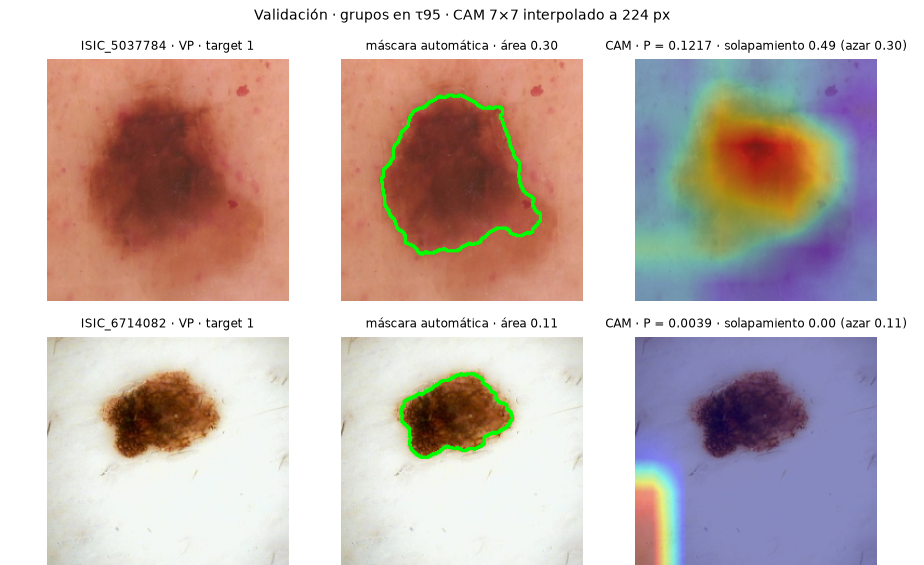
\includegraphics[width=\linewidth]{cam_tp}\\
      \nota{Dos melanomas de validación: imagen, contorno automático y mapa. Calculado con una sola red, por eso su probabilidad no es la de la página.}
    \end{column}
    \begin{column}{0.46\textwidth}
      \begin{itemize}
        \item Muestra las regiones que empujan la respuesta hacia «melanoma».
        \item Malla de $7 \times 7$ celdas: señala regiones, no estructuras finas.
        \item Depende de lo aprendido: al reiniciar los pesos de la red, el mapa cambia por completo.
      \end{itemize}
      \begin{alertblock}{Lo que se midió}
        En los melanomas detectados, solo el \textbf{22\,\%} de la activación cae dentro de la lesión; por azar sería 19\,\%.
      \end{alertblock}
    \end{column}
  \end{columns}
\end{frame}

\begin{frame}{Respaldo: sensibilidad a artefactos}
  \begin{center}
    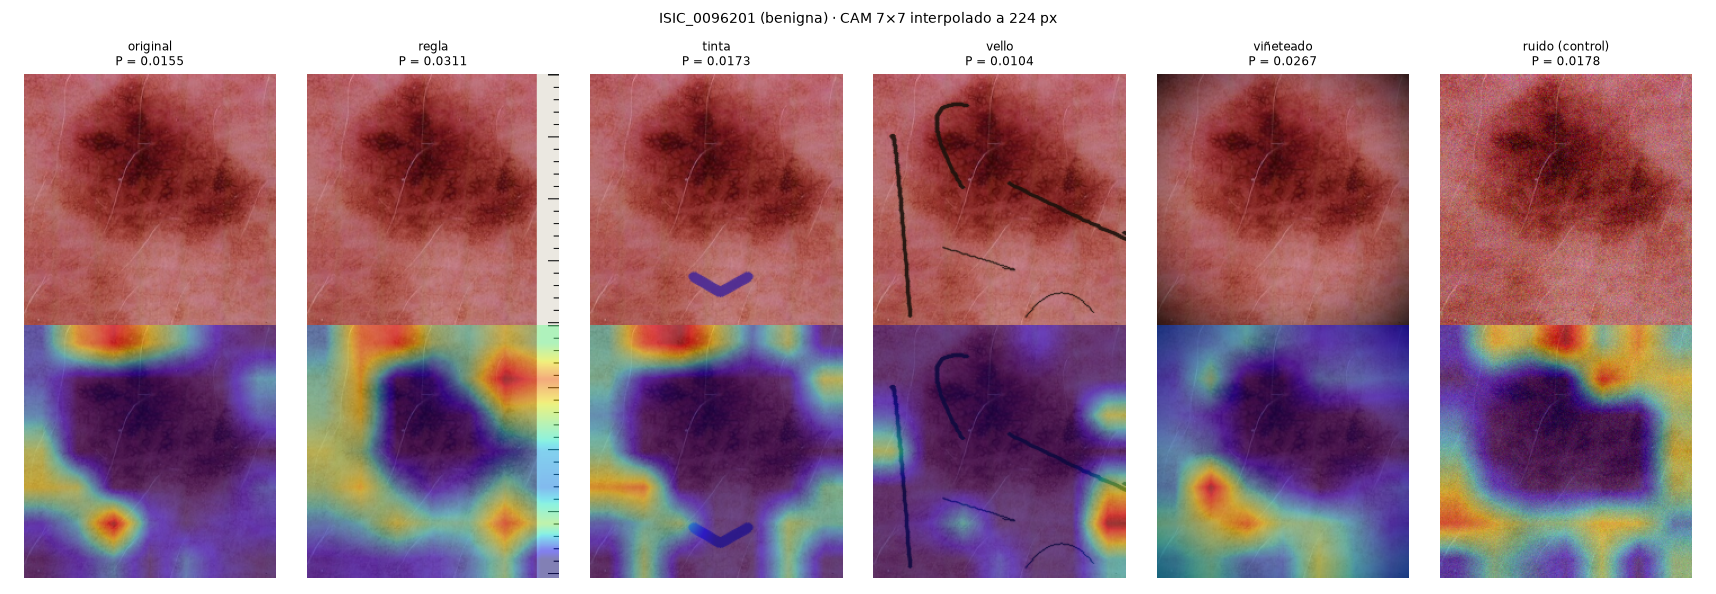
\includegraphics[width=0.74\linewidth]{f5_artifact_panel}
  \end{center}
  \vspace{-0.4em}
  \begin{columns}[T]
    \begin{column}{0.48\textwidth}
      \small
      A 1,000 lesiones benignas y 88 melanomas de validación se les añadió un artefacto sintético. Se comparó contra un control de ruido. Medido con una sola red.
    \end{column}
    \begin{column}{0.48\textwidth}
      \small
      \begin{itemize}
        \item \textbf{Tinta}: el 84\,\% de las lesiones benignas no referidas pasa a referirse (71\,\% con el control).
        \item \textbf{Vello o ruido}: 16 y 14 de 84 melanomas dejan de referirse.
      \end{itemize}
    \end{column}
  \end{columns}
\end{frame}

\begin{frame}{Respaldo: comparación con trabajos publicados}
  \begin{center}
    \small
    \begin{tabular}{lcl}
      \toprule
      \textbf{Referencia} & \textbf{AUC-ROC} & \textbf{Condiciones} \\
      \midrule
      Ha y colaboradores (2020), ganador del reto & 0.949 & 18 redes, hasta 896 píxeles, datos de 3 años \\
      Cassidy y colaboradores (2022) & 0.80 & Una red, ISIC 2020 sin duplicados \\
      \textbf{Este proyecto} & \textbf{0.843} & 3 redes a 224 píxeles, solo ISIC 2020 \\
      \bottomrule
    \end{tabular}
  \end{center}
  \vspace{0.6em}
  \begin{itemize}
    \item Los conjuntos de evaluación \textbf{no son los mismos}: la comparación ubica, no clasifica.
    \item El ganador del reto usó 18 redes, datos de tres años y resoluciones cuatro veces mayores.
  \end{itemize}
\end{frame}

\begin{frame}{Respaldo: limpieza de los datos}
  \begin{columns}[T]
    \begin{column}{0.48\textwidth}
      \textbf{Lo que se encontró}
      \begin{itemize}
        \item \textbf{433 grupos} de archivos idénticos, todos dentro de un mismo paciente.
        \item \textbf{18 grupos} de imágenes iguales que cruzan pacientes distintos.
        \item El 82\,\% de las imágenes no tiene subtipo registrado: son lesiones benignas.
      \end{itemize}
    \end{column}
    \begin{column}{0.48\textwidth}
      \textbf{Lo que se hizo}
      \begin{itemize}
        \item Los pacientes que comparten imágenes se repartieron \textbf{juntos}.
        \item Cada imagen quedó registrada con su huella SHA256.
        \item Resultado: \textbf{0 pacientes} en más de un conjunto.
      \end{itemize}
    \end{column}
  \end{columns}
  \vspace{0.8em}
  \begin{center}
    \small
    \begin{tabular}{lrrr}
      \toprule
      \textbf{Conjunto} & \textbf{Pacientes} & \textbf{Imágenes} & \textbf{Melanomas} \\
      \midrule
      Entrenamiento & 948 & 22,911 & 410 \\
      Validación & 568 & 4,963 & 88 \\
      Prueba & 540 & 5,252 & 86 \\
      \bottomrule
    \end{tabular}
  \end{center}
\end{frame}

\begin{frame}{Respaldo: relación con Ingeniería Física}
  \begin{block}{El proyecto se trabajó como un experimento de medición}
    Cada cifra se obtuvo con un procedimiento fijado de antemano y se reporta con su incertidumbre.
  \end{block}
  \vspace{0.4em}
  \begin{columns}[T]
    \begin{column}{0.48\textwidth}
      \begin{itemize}
        \item \textbf{Medir el ruido antes de comparar.} El mismo entrenamiento repetido dio 0.794 y 0.778: diferencias menores a 0.02 no se interpretan.
        \item \textbf{Incertidumbre en cada resultado.} Intervalos de confianza del 95\,\% por remuestreo de pacientes.
        \item \textbf{Calibración.} Como en un instrumento, la salida se ajusta contra una referencia para poder leerla.
      \end{itemize}
    \end{column}
    \begin{column}{0.48\textwidth}
      \begin{itemize}
        \item \textbf{Protocolo antes de medir.} El umbral y las reglas se fijaron antes de abrir el conjunto de prueba.
        \item \textbf{Controles.} El efecto de la tinta se comparó contra un control de ruido.
        \item \textbf{Modelado y optimización numérica.} 20.2 millones de parámetros ajustados por descenso de gradiente.
      \end{itemize}
    \end{column}
  \end{columns}
\end{frame}

\end{document}
